\title{Termination of flips}
\author{\textit{Based on a Lecture series by} Nikolaos Tsakanikas.}
\date{December 2024}
\maketitle

We will discuss the `termination of flips conjecture' in birational geometry, a
fundamental conjecture of the minimal model programme.

\subsection{About} This course on ??? was a part of a Winter
School for students and early career researchers, organised by the UK Algebraic
Geometry Network. The lectures were delivered in-person in the University of
Lancaster, and were transcribed by Parth Shimpi. These notes have undergone
several amendments and are not a verbatim recall of the lectures, therefore
discretion is advised when using this material. They are available online at
\url{https://pas201.user.srcf.net/documents/2024-ukag-flips.pdf}.
All errors and corrections should be communicated to by email to
\url{parth.shimpi@glasgow.ac.uk}.

\section{Birational equivalence}
Recall two varieties \(X,Y\) are said to be \emph{birational} or
\emph{birationally equivalent} if any of the following equivalent conditions
hold.
\begin{enumerate}
    \item There exists a birational map \(X\dashrightarrow Y\), i.e.\ a dominant
rational map \(X\dashrightarrow Y\) with a dominant rational inverse
\(Y\dashrightarrow X\).
\item There exist dense open subsets \(U\subseteq X\), \(V\subseteq Y\) such
that \(U\) is isomorphic to \(V\).
\item The varieties \(X,Y\) have isomorphic function fields, i.e.\ there is an
isomorphism of \(\mathbb{C}\)--algebras \(\mathbb{C}(X)\cong \mathbb{C}(Y)\).
\end{enumerate}

\begin{example}[A cuspidal cubic curve]
Consider \(C=\mathbb{V}(y^3-x^2)\) as a subset of \(\mathbb{A}^2\). The map
\(f:\mathbb{A}^1\to C\) given by \(t\mapsto (t^3,t^2)\) is a birational morphism
which restricts to an isomorphism \(\mathbb{A}^1\setminus\{0\}\isoto
C\setminus\{(0,0)\}\)
\end{example}

\begin{example}[Blowing up \(\mathbb{A}^2\) at the origin]
The space \(X\subset \mathbb{A}^2\times \mathbb{P}^1\) consisting of all points
\((x,y,[u:v])\) such that \(xv-yu=0\), called the \emph{total space of the
blowup}, admits a birational map \(\varphi:X\to \mathbb{A}^2\) given by
restricting the projection \(\mathbb{A}^2\times\mathbb{P}^1\to \mathbb{A}^2\).
The map \(\varphi\) gives an isomorphism \(X\setminus\varphi^{-1}(0)\to
\mathbb{A}^2\setminus\{0\}\), and the \emph{exceptional curve}
\(E=\varphi^{-1}(0)\subset X\) is isomorphic to a \(\mathbb{P}^1\) which
parametrises lines in \(\mathbb{A}^2\) passing through \(0\). Namely, the line
\(\ell\subset\mathbb{A}^2\) with parametric equation \((x,y)=(a_1t,a_2t)\) for
\((a_1,a_2)\neq (0,0)\) corresponds to the point \((0,0,[a_1:a_2])\in E\) where
the \emph{strict transform} \(\tilde\ell =
\overline{\varphi^{-1}(\ell\setminus\{0\}})\) meets \(E\).

Compute the strict transform of a nodal cubic.
\end{example}

\section{Classification of algebraic varieties}
Classification of varieties up to birational equivalence, i.e.\ finding a `good
representative' in every birational equivalence class, is a fundamental problem
in algebraic geometry. Minimal model program (MMP)-- define good, ask how
representatives are related, find moduli if possible. o

\subsection{Curves} Every birational equivalence class of curves contains a
unique smooth representative, which is projective. The \emph{genus} (defined as
\(g(C)=\hh^0(C,\omega_C)\)) is a discrete birational invariant which we can use
to describe birational classes. The classification takes the following shape.

\begin{tabular}{|cccc|}
    C & \(\mathbb{P}^1\)  & elliptic curves & curves of general type \\
    genus & 0 & 1 & \(\geq 1\) \\
    \(\deg(K_C)\)  & \(<0\) & 0 & \(>0\) \\
    Kodaira dimension \(K(C,K_C)\) & \(-\infty\) & 0 & 1
\end{tabular}

This trichotomy will appear later.

\section{Surfaces} Inspired by curves, one might consider smooth projective
surfaces as the good representatives of birational classes. This fails for the
following reason.

\begin{theorem}
Let \(T\) be a smooth projective surface, and \(p\in T\) a point. Then the
surface \(S\) obtained as the blow up \(\mu:S\to T\) of \(T\) in \(p\) has the
following properties.

\begin{enumerate}
\item S is a smooth projective surface.
\item \(S\setminus \mu^{-1}(p)\) is isomorphic to \(T\setminus p\).
\item \(E=\mu^{-1}(p)\) is isomorphic to \(\mathbb{P}^1\), and has
self--intersection \(E^2=-1\).
\item \(\Pic(S)\cong \mu^{\ast}\Pic(T)\oplus\mathbb{Z}\cdot E\)
\end{enumerate}
\end{theorem}

\begin{exercise}
Show that a reduced irreducible curve \(E\) inside a smooth projective surface
\(S\) is a \(-1\) curve if and only if \(E^2<0\) and \(E\cdot K_S<0\).
\end{exercise}

\begin{theorem}[Castelnuovo's contraction theorem]
If \(S\) is a smooth projective surface containing a \((-1)\)--curve \(E\), then
there exists a smooth projective surface \(T\) and a morphism \(\mu:S\to T\)
called the \emph{contraction of \(E\)} such that \(\mu(E)\) is a point \(p\in
T\) and \(S\setminus E\) is isomorphic to \(T\setminus \{p\}\).  In fact,
\(\mu\) is the blow up of \(T\) in \(p\).
\end{theorem}

We can use this to find good representatives in a given birational class via the
following algorithm.

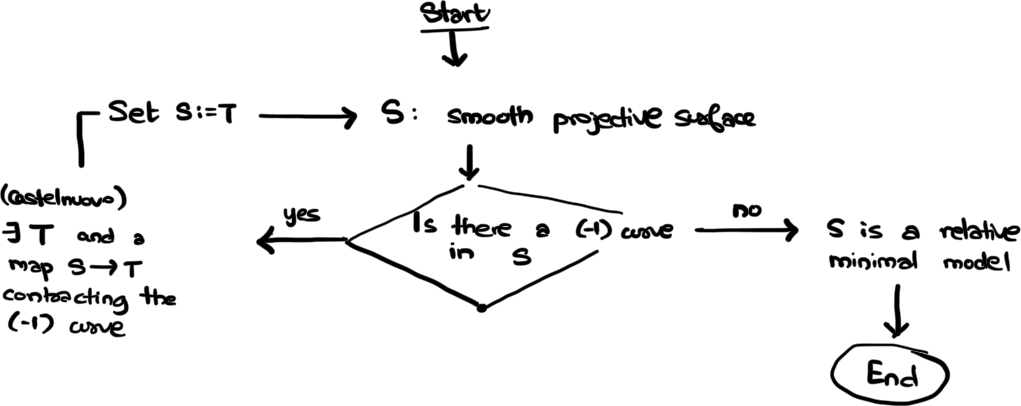
\includegraphics[width=0.5\textwidth]{images/surface_MMP.png}

This process terminates, since the Picard rank drops by \(1\) after every
contraction. The outcome of this procedure can be any of the following:
\begin{enumerate}
\item \(\mathbb{P}^2\), i.e.\ the del Pezzo surface of degree \(9\).
\item Minimal geometrically ruled surfaces \(S\), which are
\(\mathbb{P}^1\)--bundles over \(C\).
\item Minimal models, which are characteristed by having non--negative Kodaira
dimension.
\end{enumerate}

The first two cases are characterised by having Kodaira dimension \(-\infty\),
and are the so-called \emph{Mori fiber spaces}. Their birational classes may
have multiple good representatives, Sarkisov program.

\subsection{MMP in dimension \(\geq 3\)} Given a smooth variety \(X\), we expect
a sequence of birational surgery operations which produce a (possibly mildly
singular) variety \(Y\) which comes equipped with a fibration \(f:Y\to Z\)
(projective surjective morphism with connected fibers). We again have a
dichotomy--

\begin{enumerate}
\item if \(X\) is uniruled (i.e.\ covered by rational curves), then
\(f:Y\to Z\) is a Mori fiber space and satisfies \(\dim Z < \dim Y\) with
relative Picard rank \(1\) and the general fiber \(F\) is a Fano variety with
terminal singularities. Conjecturally this is the case of negative Kodaira
dimension, and is proven for dimension \(\leq 3\).

\item If \(X\) is not uniruled then we obtain a variety \(Y\) called a
\emph{minimal model}, which has nef canonical class. The existence of \(f:Y\to
Z\) is predicted by the \emph{abundance conjecture}, which asserts that
the linear system \(|mK_Y|\) is non--empty and basepoint free for some
\(m\in \mathbb{N}\). If \(F\)is a general fiber of \(f\), then the Iitaka
fibration theorem says that \(K_F\) is trivial i.e.\ \(F\) is a Calabi Yau
variety and further, \(Z\) is a canonically polarised variety i.e.\ \(K_Z\) is
ample.
\end{enumerate}

THe MMP thus predicts that there are three building blocks in birational
geometry-- Fano varieties, Calabi--Yau varieties, and canonically polarised
varieties. For hypersurfaces in \(\mathbb{P}^N\), these correspond to degrees
\(\leq N, =N+1, \geq N+2\) respectively.

\begin{exercise}
    If \(C\) is a smooth projective curve of genus \(\geq 2\), show that
    \(\hh^0(C, mK_C)=(2m-1)(g-1)\) for \(m\geq 2\).
\end{exercise}

\begin{exercise}
    If \(S\) is a minimal smooth projective surface of Kodaira dimension \(2\),
    show that \(\hh^0(X,mK_S)=\frac{1}{2}m(m-1)K_S^2+\chi(\OO_S)\)
\end{exercise}

\section{Preliminaries}
\subsection{Canonical class} If \(X\) is a smooth variety of dimension \(n\),
then have a cotangent bundle \(\Omega^1_X\) and the canonical bundle
\(\omega_X=\Exter^n\Omega^1\). The canonical class \(K_X\) is any divisor such
that \(\omega_X=\OO_X(K_X)\).

\(K_X\) makes sense even if \(X\) is just normal, by taking the canonical class
of the smooth locus and extending (uniquely) by Hartog's lemma. This is a Weil
divisor, well-defined up to linear equivalence.

\subsection{Iitaka dimension} If \(X\) is a projective variety and \(L=\OO(D)\)
is a line bundle, then we wish to understand the asymptotic behaviour of
\(\hh^0(L^n)\). Base locus of \(L\) is the set of all points in \(X\) where
every global section of \(L\) vanishes, then have a map
\[
    \varphi =\varphi_{|L|}:X\setminus\text{Base}|L| \to
    \mathbb{P}\HH^0(X,L).
\]

Write \(\mathbb{N}(L)\) for the set of all \(m\) for which \(\HH^0(X,L^m)\neq
0\). If \(m\in \mathbb{N}(L)\) then have a rational map \(\varphi_{|L^m|}\) with
image \(Y_m\).

\begin{definition}
For \(X,L\) as above and \(X\) normal, the Iitaka dimension of \(L\) is defined
as
\[\kappa(X,L)=\begin{cases}
\max_m(\dim Y_m), &\mathbb{N}(L)\neq \{0\}\\
-\infty, &\mathbb{N}(L)=\{0\}.
\end{cases}\]

Thus \(\kappa(X,L)\in \{-\infty, 0,1,...,\dim X\}\). If \(X\) is a smooth
projective variety, then \(\kappa(X)=\kappa(X,\omega_X)\) is called the Kodaira
dimension of \(X\).
\end{definition}

\begin{remark}
If \(\kappa(X,L)=k\) then \(\dim\varphi_m(X)=k\) for all sufficiently large
\(m\in \mathbb{N}(L)\). In particular, \(k=0\) if and only if \(\hh^0(X,L^m)\leq
1\) for all \(m\) and \(\hh^0(X,L^n)=1\) for some \(n>0\).
\end{remark}

\begin{remark}
If \(\kappa(X,L)=k\) then there exist \(\alpha,\beta>0\) such that \(\alpha m^k
\leq \hh^0(X,L^m) \leq \beta m^k\)  for sufficiently large \(m\in
\mathbb{N}(L)\).
\end{remark}

THe definition also makes sense for \(\mathbb{k}\)--Cartier
\(\mathbb{k}\)--divisors for \(\mathbb{k}\in \{\mathbb{Q},\mathbb{R}\}\), by
rounding down \(mD\) when taking global sections.

\begin{remark}
If \(f:Y\to X\) is a surjective morphism between normal varieties and \(D\) is a
\(\mathbb{Q}\)--cartier \(\mathbb{Q}\)--divisor on \(X\) then
\(\kappa(X,D)=\kappa(Y,f^\ast D)\).

If \(f:Y\to X\) is a projective birational morphism between normal varieties and
\(D\) is a \(\mathbb{Q}\)--cartier \(\mathbb{Q}\)--divisor on \(X\), then for
every effective \(f\)--exceptional divisor \(E\subset Y\) we have
\(\kappa(X,D)=\kappa(Y,f^\ast D+E)\).
\end{remark}

\subsection{Notions of positivity}
Let \(X\) be a normal projective variety, and \(L=\OO(D)\) a line bundle on
\(X\). Then \(L\) is \emph{globally generated} if \(\text{Base}|L|=\emptyset\),
equivalently if the natural map \(\OO\otimes \HH^0(X,L)\to L\) is surjective,
equivalently if the rational map \(\varphi_{|L|}\) is a morphism.

\(L\) is semiample if there is some \(m>0\) such that \(L^m\) is globally
generated.

\(L\) is ample if there is some \(m>0\) such that \(L^m\) is globally
generated and \(\varphi_{|L^m|}\) is an embedding.

\(L\) is nef if \(\int_{C} \cc_1(L)\geq 0\) for every irreducible curve
\(C\subset X\), equivalently if \(D\cdot C \geq 0\) for every irreducible curve
\(C\subset X\).

\(L\) is big if \(\kappa(X,L)=\dim X\). Then \(D\) is big iff and only if there
is an \(m>0\) such that \(mD=A+E\) for \(A\) ample and \(E\) effective. Then
\(\varphi_{|mD|}\) is birational.

\(D\) is pseudoeffective if \([D]=\lim_{k\to \infty}[E_k]\) for \([E_k]\) a
sequence of effective divisors in \(\text{NS}(X)\).


We have the following.
\[
\text{ample}\Rightarrow \text{semiample}\Rightarrow \text{nef}\Rightarrow
\text{pseudoeffective},\qquad \text{ample}\Rightarrow \text{big}\Rightarrow
\text{pseudoeffective}.
\]

We consider the following real vector spaces-- the Neron Severi space
\(\text{N}^1(X)_\mathbb{R} = \text{Div}(X)/\text{numerical equivalence} \otimes
\mathbb{R}\) is finite dimensional and its dimension \(\rho(X)\) is the Picard
number of \(X\). \(\text{N}_1(X)_\mathbb{R}=\text{Z}_1(X)/\equiv \otimes
\mathbb{R}\) is the realification of group of numerical equivalence classes of
1-cycles.

Consider the cones \(\text{Amp}(X), \text{Nef}(X), \text{Big}(X),
\overline{\text{Eff}}(X)\). We know that the nef cone is the closure of the
ample cone and the ample cone is the interior of the nef cone. Likewise the
closure of the big cone is the pseudoeffective cone, and the interior of the
pseudoeffective cone is the big cone.

Inside \(N_1(X)_\mathbb{R}\) have \(NE(X)\) generated by classes of irreducible
curves, and its closure \(\overline{NE}(X)\) the Kleiman--Mori cone.

\begin{exercise}
Let \(S\) be a smooth projective surface with Kodaira dimension \(\geq 0\). Show
that \(S\) contains no \((-1)\)--curves if and only if \(K_S\) is nef.
\end{exercise}

\section{The MMP in arbitrary dimensions}
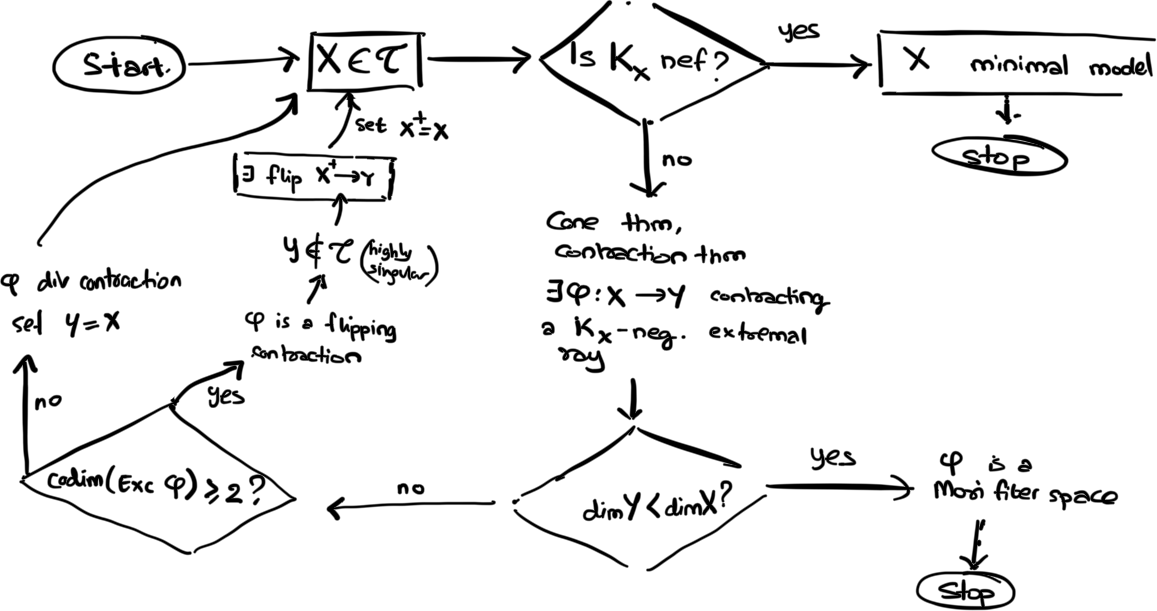
\includegraphics[width=\textwidth]{images/general_MMP.png}

Existence of flips has been solved in ``full generality'' (2019), Mori got
fields medal ('90s) for proving the existence of flips of terminal 3-folds.

Question: does the procedure terminate? Whenever we have a divisorial
contraction \(\varphi:X\to Y\), the Picard rank drops so we can only have
finitely many divisorial contractions when running the MMP. Flipping
contractions preserve the Picard rank.

Conjecture (termination of flips): there can only appear finitely many flips
when running the MMP.

The MMP has been established in full generality in dimension \(3\) in the 80s
and 90s by the works of Kawamata, Mori, Ried, Shokurov, and many others.

The MMP studies pairs (objects of form \(X,B\)) which offer flexibility and
are great for inductive purposes, and generalised pairs \((X,B+M)\)

Pseudoeffectivity of \(K_X\) determines whether or not you get minimal model or
a Mori fiber space.

\subsection{Cone and contraction theorems}
Cone theorem: The Kleiman mori cone \(\overline{\NumEff}(X)\) is the sum of the
\(K_X\)--non-negative part and the span of \(K_X\)--negative extremal rays
\(\sum_i \mathbb{R}_{\geq 0}[\gamma_i]\) where each \(\gamma_i\subseteq X\) is
an irreducible rational curve. This relies on characteristic \(p\) methods
(Mori's bend and break technique). Further for any \(\varepsilon>0\), there
are finitely many \(\gamma_i\) with \(K_X\cdot \gamma_i > \varepsilon\). But may
have accummulation near the hyperplane \(K_X=0\).

Contraction theorem: every \(K_X\)--negative extremal ray \(R\) can be
contracted by a morphism \(\varphi:X\to Y\), \(\varphi_\ast \OO_X=\OO_Y\), and
where a curve \(C\subset X\) is contracted by \(\varphi\) if and only if
\([C]\in R\).

\section{Pairs and their singularities} If \(X\) is a smooth variety, a reduced
\(\mathbb{Q}\)--divisor \(D=\sum D_i\) is SNCif each \(D_i\) is smooth and all
components intersect transversally. If not reduced then we say it is SNC when
the underlying reduced divisor is so.

A resolution of \(X\) is a projective birational morphism \(g:Y\to X\) where
\(Y\) is smooth.

\(X\) a variety, \(D\) a \(\mathbb{Q}\)--divisor on \(X\). A log--resolution of
\((X,D)\) is a projective birational morphism \(g:Y\to X\) from a smooth variety
\(Y\) such that the exceptional locus of \(g\) is a divisor and \(Exc(g)\cup
\tilde{D}\) has SNC support.

Theorem (Hironaka) Log resolutions exist over fields of characteristic \(0\).

\(X\) a variety, \(f:Y\to X\) a projetive birational morphism from \(Y\) normal.
\(E\subset Y\) prime divisor. Then we say \(E\) is a divisor over \(X\) and
\(f(E)\) is called the center of \(E\) on \(X\), written \(\cc_X(E)\).
Divisorial valuations of \(k(X)\)?

\begin{definition}
    A pair \((X,B)\) consists of a normal variety \(X\) together with an
    effective \(\mathbb{Q}\)--divisor \(B\) on \(X\) such that \(K_X+B\) is
    \(\mathbb{Q}\)--cartier.
\end{definition}

\begin{definition}
    If \(X\) is a normal variety and \(B\) is a \(\mathbb{Q}\)--divisor on \(X\)
    such that \(K_X+B\) is \(\mathbb{Q}\)--cartier. If \(f:Y\to X\) is a
    resolution, pick canonical divisors \(K_Y,K_X\) such that \(f_\ast
    K_Y=K_X\). Then \(K_Y=f^\ast (K_X+B) + \sum a(E_i, x, B)E_i\). The rational
    number \(a(E_i,x,B)\) is called the discrepancy of \(E_i\) with respect to
    \((X,B)\). Note \(f^{-1}B\) always has discrepancy \(1\).
\end{definition}

The discrepancy of \((X,B)\) is defined as the infimum of all discrepancies
\(a(E,X,B)\) where \(E\)is a prime divisor over \(X\) which is exceptional.

The total discrepancy of \((X,B)\) is the defined as the infimum of all
discrepancies \(a(E,X,B)\) for all prime divisors \(E\) over \(X\).

Every divisor on \(X\) other than \(B\) has discrepancy zero by definition.

\begin{exercise}
    Let \(X\) be a smooth variety and let \(B=\sum a_iD_i\) be a
    \(\mathbb{Q}\)--divisor on \(X\). Let \(Z\subset X\) be a closed subvariety
    of codimension \(n\), and let \(p:Y\to X\) be the blow up of \(X\) along
    \(Z\) and \(E\subset Y\) the component of exceptional divisor dominating
    \(Z\). Show that \(a(E,X,B)=r-1-\sum a_i\text{mult}_Z(D_i)\).
\end{exercise}

\begin{exercise}
    Let \(f:Y\to X\) bea  proper birational morphism between normal varieties.
    Let \(B_X\) resp \(B_Y\) be a \(\mathbb{Q}\)--divisor on \(X\) resp \(Y\)
    such that \(K_Y+B_Y=f^\ast (K_X+B_X)\) and \(f_\ast B_Y=B_X\). Show that for
    any divisor \(F/X\) we have \(a(F,X,B_X)=a(F,Y,B_Y)\).
\end{exercise}

\begin{lemma}
    If \((X,B)\) is as before, then either \(discrep(X,B)=-\infty\) or
    \(-1\leq totaldiscrep(X,B)\leq discrep(X,B) \leq 1\).

    If \((X,B=\sum a_i D_i)\) is a log--smooth pair (ie \(X\) smooth and \(B\)
    has SNC support) then \(discrep(X,B)=\min\{1,\min\{1-a_i\},\min_{D_i\cap
    D_j\neq \emptyset}\{1-a_i-a_j\}\}.\)
\end{lemma}

\begin{definition}[Singularities of pairs]
    We say a pair \((X,B)\) is terminal if \(discrep(X,B)>0\), canonical if
    \(discrep(X,B)\geq 0\), klt if \(discrep(X,B)> -1\) and \(\lfloor B
    \rfloor=0\), and log canonical if \(discrep(X,B)\geq -1\).
\end{definition}

\begin{proposition}
    Let \(X\) be a normal variety such that \(K_X\) is \(\mathbb{Q}\)--cartier.
    Let \(f:Y\to X\) be a resolution. Write \(K_Y=f^\ast K_X + \sum a_iE_i\).
    Then \(X\) is canonical if and only if \(a_i\geq 0\) for all \(i\), and
    \(X\) is terminal if and only if \(a_i > 0\) for all \(i\).
\end{proposition}

\begin{proposition}
    Let \((X,B)\) be a pair, \(B\) not necessarily effective. Let \(f:Y\to X\)
    be a log resolution. Suppose \(K_Y+f^{-1}B = f^\ast(K_X+B)+\sum a_i E_i\).
    Then \((X,B)\) is klt if and only if \(a_i >-1\), and  log canonical iff
    \(a_i\geq -1\).
\end{proposition}

\begin{exercise}
 Let \(X=\mathbb{A}^2\) and \(B=\text{div}(x^2-y^3)\). The pair \((X, dB)\) is
 KLT (resp.\ log canonical) iff \(0\leq d < 5/6\) (resp.\ \(0\leq d \leq 5/6\)).
\end{exercise}

\begin{lemma}[Negativity lemma]
    Let \(h:Z\to Y\) be a proper birational morphism. Let \(D\) be a
    \(\mathbb{Q}\)--cartier \(\mathbb{Q}\)--divisor on \(Z\) such that \(-D\) is
    \(h\)--nef. Then \(D\geq 0\) if and only if \(h_\ast D \geq 0\).
\end{lemma}

\begin{exercise}
Consider a commutative diagram

\[\begin{tikzcd}
    X \arrow[rr,dashrightarrow, "\varphi"] \arrow[dr, "f"'] && X' \arrow[dl,
    "f'"] \\
    &Y&
\end{tikzcd}\]
for \(X,X'\) normal varieties and \(f,f'\) projective birational. Let \(B,B'\)
be \(\mathbb{Q}\)--divisors on \(X,X'\) respectively. Assume \(f_\ast B=f'_\ast
B'\), \(-(K_X+B)\) is Q-cartier and f-nef, \(K_X+B'\) is Q-cartier and f'-nef.
Show that every exceptional divisor \(E/Y\) we have \(a(E,X,B)\leq a(E,X',B')\)
and show that the strict inequality holds if either \(-(K_X+B)\) is \(f\)--ample
and \(f\) is not an isomorphism above generic point of \(c_Y(E)\), or
\(K_{X'}+B'\) is \(f'\)--ample and \(f'\) is not an iso above geneirc of cY(E).

This models divisorial contractions and flips, so MMP doesnt make singularities
worse.
\end{exercise}

\begin{definition}
    Let \(X,B\) be a pair. A \((K_X+B)\)--flipping contraction is a proper
    birational morphism \(\theta:X\to W\) such that the codimension of
    exceptional locus is \(\geq 2\) and \(-K_X+B\) is \(\theta\)--ample.

    A pair \((X^+,B^+)\) together with a proper birational morphism
    \(\theta^+:X^+\to W\) is called a \((K_X+B)\)--flip of \(\theta\) if codim
    of exceptional \(\theta^+\) is \(\geq 2\) and \(K_{X^+}+B^+\) is
    \(\theta^+\)--ample.
\end{definition}

\begin{remark}
    If a variety \(X\) is terminal then it is smooth in codimension \(2\) i.e.\
    the singular locus has codimension \(\geq 3\). Thus terminal surfaces are
    smooth. Further if \((X,B)\) is terminal then \(\lfloor B \rfloor = 0\).
\end{remark}

\begin{definition}
    Let \((X,B=\sum a_i D_i)\) be a pair and \(0\leq a_i \leq 1\) for all \(i\).
    Then \((X,B)\) is dlt (divisorially log terminal) if there is a closed
    subset \(Z\subset X\) such that
    \begin{enumerate}
        \item \((X\setminus Z, B|_{X\setminus Z})\) is log--smooth
        \item If \(f:Y\to X\) is a birational morphism and \(E\subset Y\) is a
            prime divisor with \(\cc_X(E)\subset Z\) then \(a(E,X,B)>-1\).
    \end{enumerate}
\end{definition}

Thus dlt implies log canonical, and dlt is klt iff \(\lfloor B \rfloor = 0\).
DLT is KLT away from log--smooth locus.

\section{Flips and termination}
\begin{definition}
    For \((X,B)\) a pair, a \(K_X+B\)--flipping contraction is a proper
    birational morphism \(\theta:X\to W\) such that
    \(\text{codim}(\text{Exc}(\theta))\geq 2\) and \(-(K_X+B)\) is
    \(\theta\)--ample. In this case a pair \((X^+, B^+)\) with a proper
    birational morphism \(\theta^+:X^+\to W\) is called a \((K_X+B)\)--flip if
    \(\text{codim}\text{Exc}(\theta^+)\geq 2\) and \(K_{X^+}+B^+\) is
    \(\theta^+\)--ample.

    In this case \(B^+\) is the strict transform of \(B\).
\end{definition}

If a flip exists then it has to be unique, and \(X^+=\Proj_W\bigoplus_{m\geq
0}\theta_\ast \OO_X(m(K_X+B))\). The existence of flips is equivalent to the
ring being finitely generated, and the question has been settled in full
generality (Mori '88 showed this for terminal 3-folds, Shokurov '92 proved the
existence for KLT pairs, Kollar et al (book Geometry of algebraic 3-folds)
showed existence of log canonical pairs in dimension 3, BCHM '10 showed the
existence of flips for KLT pairs of any dimension, Birkar '12 and Hacon-Xu '13
showed existence of flips for LC pairs in any dimension. All of this for
relative Picard rank 1, general by ???)

\begin{lemma}[(monotonicity)]
    Let \((X,B)\dashrightarrow (X^+,B^+)\) be a \((K_X+B)\) flip over \(W\). For
    any divisorial valuation \(F/X\) we have \(a(F,X,B)\leq a(F,X^+,B^+)\) and
    the strict inequality holds if and only if either \(\cc_X(F)\subseteq
    \text{Exc}(\theta)\) or \(\cc_{X^+}(F)\subset \text{Exc}(\theta^+)\).
\end{lemma}

\begin{lemma}
    have \(\dim(\text{Exc}\theta)+\dim(\text{Exc}\theta^+)\geq \dim X - 1\).
    Thus in dimension \(3\), the only possibility is that a bunch of curves get
    flipped to a bunch of curves. In dimension 4, all combinations
    \((2,1),(1,2),(2,2)\) are possible.
\end{lemma}

\begin{lemma}
    For \((X,B)\) a log canonical pair, if \(X\) is \(\mathbb{Q}\)--factorial
    then so is \(X^+\) and further, the Picard rank is preserved.
\end{lemma}

(STATES THE TERMINATION OF FLIPS CONJECTURE)

Shokurov '85 proved that the conjecture holds for terminal 3-folds with no
boundary. Kawamata '92 showed that the conjecture holds for
\(\mathbb{Q}\)--factorial dlt 3-folds. Shokurov '96 showed that conjecture holds
for LC pairs in dimension 3. Kawamata--Matsuda--Matsuki '87 showed conjecture
holds for terminal 4-folds (no boundary). Fujino '04--'05 showed that conjecture
holds for canonical pairs of dimension 4. Alexeev--Hacon--Kawamata '07 showed
conjecture holds for klt pairs of dimension 4 with \(-K_X-B\equiv E\geq 0\).
Birkar '10 showed that the conjecture holds for KLT pairs of dimension 4 with
Kodaira dimension of \(K_X+B\) at least 2. Hacon--Moraga '20, Chen--Tsakanikas
'23 show that the conjecture holds for LC pairs \((X,B)\) of dimension 4 such
that \(K_X+B\) is pseudoeffective. Lenn--Pacienza '10 show that any MMP starting
from an IHS pair (i.e.\ log canonical pair with underlying smooth IHS variety)
terminates. Denisi--Ortiz--Tsakanikas--Xie '24 show that any MMP starting from
an Enriques pair (log canonical pair with underlying smooth Enriques manifold) terminates.

\subsection{Shokurov's proof} He defines a special invariant.

\begin{definition}
    If \(X\) is a normal projective with terminal singularities, then the
    difficulty of \(X\) is the number of \(E\) exceptional over \(X\) such that
    \(a(E,X,0)<1\).
\end{definition}
He shows this is well--defined (finite) and upon flipping, it does not increase.

Thus it suffices to show that the difficulty decreases after a flip. This is
true in dimension \(3\). We know \(X^+\) is terminal, so \(X^+\) is smooth at
the generic point of every flipped curve. Pick such a \(C^+\) and blow up
\(X^+\) at the generic point of this curve, and denote by \(E^+\) the
exceptional divisor dominating \(C^+\). Then [Exercise] show that
\(a(E^+,X,0)<a(E^+,X^+,0)\) since center of \(E^+\) lies in the flipped locus.
But \(a(E^+,X^+,0)=1\), so the difficulty of \(X\) is bigger than that of
\(X^+\).

In dimension 4, if the flipping and flipped loci have dimensions \((1,2)\) or
\((2,2)\) then again difficulty decreases. But \((2,1)\) needs a different
method.

\subsection{Very rough sketch of Chen--Tsakanikas} it is a special case of the
folowing more general statement:
\begin{theorem}
    Assume termination of flips for klt generalised pairs of dimension \(\leq
    n-1\). Let \((X,B+M)\) be a log canonical generalised pair of dimension n
    such that \(K_X+B+M\) is pseudoeffective. If \((X,B+M)\) has a minimal model
    then any sequence of flips starting from \((X,B+M)\) terminates. (If some
    MMP terminates then all MMPs terminate).
\end{theorem}

Main ideas are special termination and ascending chain condition for log
canonical thresholds proved by (Hacon--McKernan--Xu).
